\documentclass{sigchi}

% Remove or comment out these two lines for final version
\toappearbox{\Large Submitted to CSCW'14. \\Do not cite, do not circulate.}
\pagenumbering{arabic}% Arabic page numbers for submission. 

% Use \toappear{...} to override the default ACM copyright statement (e.g. for preprints).

% Load basic packages
\usepackage{balance}  % to better equalize the last page
\usepackage{graphics} % for EPS, load graphicx instead
\usepackage{times}    % comment if you want LaTeX's default font
\usepackage{url}      % llt: nicely formatted URLs
\usepackage{listings}
\usepackage{gensymb}
\usepackage{multirow}
\usepackage{color}
\usepackage{algorithmic}     % For algorithm pseudocode
\usepackage{multirow}
%\usepackage{caption}
%\usepackage{subcaption}

% llt: Define a global style for URLs, rather that the default one
\makeatletter
\def\url@leostyle{%
  \@ifundefined{selectfont}{\def\UrlFont{\sf}}{\def\UrlFont{\small\bf\ttfamily}}}
\makeatother
\urlstyle{leo}


% To make various LaTeX processors do the right thing with page size.
\def\pprw{8.5in}
\def\pprh{11in}
\special{papersize=\pprw,\pprh}
\setlength{\paperwidth}{\pprw}
\setlength{\paperheight}{\pprh}
\setlength{\pdfpagewidth}{\pprw}
\setlength{\pdfpageheight}{\pprh}


% create a shortcut to typeset table headings
\newcommand\tabhead[1]{\small\textbf{#1}}


%************* Andreas Additions
%% Usage: You do not need \begin{enumerate} and \end{enumerate} statements.
%% Just the \squishlist and \squishend statements, and the \items's in between.
%% If you do not want a bulleted list, you can add " [(a)]" after the fist \item,
%% " [(b)]" after the second one, etc, to get a, b, ... bullets...
%% (or 1, 2, 3... can replace the a, b, c...)

\newcommand{\squishlist}{
 \begin{list}{$\bullet$}
 {
  \setlength{\itemsep}{0pt}
  \setlength{\parsep}{0pt}   %3pt
  \setlength{\topsep}{0pt}   %3pt
  \setlength{\partopsep}{0pt}
  \setlength{\leftmargin}{1.5em}
  \setlength{\labelwidth}{1em}
  \setlength{\labelsep}{0.5em} } }

\newcommand{\squishend}{
  \end{list}  }

% Alter some LaTeX defaults for better treatment of figures:
    % See p.105 of "TeX Unbound" for suggested values.
    % See pp. 199-200 of Lamport's "LaTeX" book for details.
    %   General parameterbnos, for ALL pages:
    \renewcommand{\topfraction}{0.9}	% max fraction of floats at top
    \renewcommand{\bottomfraction}{0.8}	% max fraction of floats at bottom
    %   Parameters for TEXT pages (not float pages):
    \setcounter{topnumber}{2}
    \setcounter{bottomnumber}{2}
    \setcounter{totalnumber}{4}     % 2 may work better
    \setcounter{dbltopnumber}{2}    % for 2-column pages
    \renewcommand{\dbltopfraction}{0.9}	% fit big float above 2-col. text
    \renewcommand{\textfraction}{0.07}	% allow minimal text w. figs
    %   Parameters for FLOAT pages (not text pages):
    \renewcommand{\floatpagefraction}{0.7}	% require fuller float pages
	% N.B.: floatpagefraction MUST be less than topfraction !!
    \renewcommand{\dblfloatpagefraction}{0.7}	% require fuller float pages

	% remember to use [htp] or [htpb] for placement


% Adds a space between the text and the [T]op \hline
% Must use the \T *within* a cell, not right after the \hline
\newcommand\T{\rule{0pt}{2.5ex}}%{3.1ex}}

% Adds a space between the text and the [B]ottom \hline
% Must use the \B *within* a cell, not right after the \hline
\newcommand\B{\rule[-1ex]{0pt}{0pt}}%[-1.7ex]{0pt}{0pt}}

% Enable grayed-out text environments, like {\graytext foo}:
\definecolor{gray}{RGB}{163,163,163}
\newenvironment{graytext}{\color{gray}}{\ignorespacesafterend}

%\setlength{\belowcaptionskip}{-3pt}

%************* End Andreas Additions


% Make sure hyperref comes last of your loaded packages, 
% to give it a fighting chance of not being over-written, 
% since its job is to redefine many LaTeX commands.
\usepackage[pdftex]{hyperref}
\hypersetup{
pdftitle={SIGCHI Conference Proceedings Format},
pdfauthor={LaTeX},
pdfkeywords={SIGCHI, proceedings, archival format},
bookmarksnumbered,
pdfstartview={FitH},
colorlinks,
citecolor=black,
filecolor=black,
linkcolor=black,
urlcolor=black,
breaklinks=true,
}


% End of preamble. Here it comes the document.
\begin{document}

\title{EchoTree: Engaged Conversation when Capabilities are Limited}

% Note that submissions are blind, so author information should be omitted


%\numberofauthors{2}
%\author{
%  \alignauthor Andreas Paepcke\\
%    \affaddr{Stanford University}\\
%    \affaddr{Stanford, CA}\\
%    \email{paepcke@cs.stanford.edu}
%  \alignauthor Caroline Pantofaru, Dirk Thomas, Austin Hendrix, Sarah Elliot, Sharon Marzouk\\
%    \affaddr{Willow Garage}\\
%    \affaddr{Menlo Park, CA}\\
%    \email{\{pantofaru,dthomas,ahendrix,selliott,smarzouk\}@willowgarage.com}
%    }

% \author{
%  \parbox[t]{18.0cm}{\centering 
%    {\em Andreas Paepcke\**}, 
%    {\em Caroline Pantofaru\**\**}, 
%    {\em Dirk Thomas\**\**}, 
%    {\em Austin Hendrix\**\**}, 
%    {\em Sharon Marzouk\**\**},
%    {\em Sarah Elliot\**\**}}\\
%  \\
%  \parbox[t]{5.0cm}{\centering
%         \**Stanford University\\
%         353 Serra Mall\\
%         Stanford, CA 94305\\
% 	paepcke@cs.stanford.edu}\\
%  \\
%  \parbox[t]{10.0cm}{\centering
%     	\**\**Willow Garage\\
% 	68 Willow Road\\
% 	Menlo Park, CA 94025\\
%        \{pantofaru,dthomas,ahendrix,smarzouk,selliott@willowgarage.com\}}
% }

% Teaser figure can go here
%\teaser{
%  \centering
%  \includegraphics{Figure1}
%  \caption{Teaser Image}
%  \label{fig:teaser}
%}

\maketitle

\begin{abstract}
Speech and motor-impaired individuals using assistive technologies to communicate face a common problem; the inevitable conversational 'dead space' which occurs while the user generates written or artificially-spoken sentences can dramatically reduce conversation quality and partner engagement. To address this problem, we introduce {\em EchoTree}, a visualization approach employing predictive language modeling to generate and display candidate utterances, thus allowing  partners to make guesses about the impaired user's intended conversational direction. By including partners in the process of sentence generation, EchoTree mitigates the dead space problem by (1) engaging partners in a collaborative activity, and (2) reducing the task of word-generation to that of confirming a word choice. Our implementation is browser-based, making it suitable for face-to-face or remote communication, as multiple parties can view and interact with the same stream of EchoTrees from desktops, tablets, or smartphones. We describe the visual and system design choices and the experiments with data sources and language models which led to our current implementation.
\end{abstract}

\keywords{assistive technology; prolonged engagement; collaborative conversation; story telling, game}

\category{H.5.2}{Information Interfaces And Presentation}{User Interfaces - Interaction styles}

\terms{Human Factors; Design}


\tolerance=400

%\newcommand{\degree}{$^\circ$}

\section{Introduction}
Before introducing EchoTree, we start by introducing 'Henry', a motion and speech-impaired individual who acted as both a motivation and a design partner in this endeavor. While Henry enjoys conversing, his speech impairment is complete. Quadriplegia, while severely limiting, does allow Henry to move his head in affirmation or negation, and his hand can operate a mouse button. 

One of Henry’s communication modes is a text-to-speech system ({\em tts}). This system works via a camera mounted on top of his laptop, which tracks a confetti-sized white dot pasted on the lower left of his glasses. The resulting cursor allows Henry to hunt down the keys of an onscreen keyboard. On a very good day, the resulting speed is 15 words per minute.
The tts produces sound only once a sentence has been completed; uttering words as Henry types them could work, but this approach makes it difficult for listeners to track the very slowly evolving sentence in their mind. In addition, poor tts performance for some words would further impede comprehension, which is supported by the context available when a full sentence in pronounced together.

This slow communication channel results in very frustrating experiences during gatherings like parties. A guest will make a remark to Henry, who will go to work on an answer. To the conversation partner, Henry looks frozen, peering at his laptop screen, the back surface of which reveals nothing to the expectant partner. Often, the potential conversation partner wanders off bewildered before Henry can finish his sentence. While a second display would allow a listener to understand that a response is forthcoming, such a solution would still keep listeners passive, and likely bored.

\begin{figure}
   \centering
   \includegraphics[width=0.6\columnwidth]{Figs/henryBigramsCarTree.png}
   \caption{Screenshot of an EchoTree.}
   \label{fig:echoTree}
\end{figure}

In an attempt to ameliorate this situation for users such as Henry, we have developed a collaborative visual communication approach -- {\em EchoTree}, an example of which is shown in Figure~\ref{fig:echoTree}. As the impaired typist generates written words using an existing device, such as a laptop, an underlying language model predicts the conversation threads most ‘likely’ to follow each typed word; these multiple possibilities are presented on a display using a WordTree\cite{Wattenberg2008} layout. Conversation partners can view and suggest possible sentence completions to the typist, possibly saving time and speeding the conversation.

In this paper, we present the EchoTree approach for the first time. We describe the visual design, user experience, and system architecture of our current implementation, a browser-based visualization which can be accessed from any web-enabled device, allowing for both face-to-face and remote communication. In addition, we present the results of an experiment aimed at understanding which data sources and modeling choices where best suited for generating the underlying language model. Finally, we discuss our findings, how they fit into existing knowledge about facilitating communication for users with speech and motor impairments, and opportunities for future work.

\section{User Experience}
A word tree\cite{Wattenberg2008} is read from left to right, beginning
with a single word, the {\em root}. Branching out from the root are
words that might follow the root in an underlying document
collection. EchoTree provides five out-branches, which are sorted top
to bottom by their likelihood of being the follower word to the
root. Each follower word candidate itself features five possible
followers to the candidate.  The tree thereby presents a number of
possible conversation threads that might begin with the root word.

The underlying collection, of course, impacts the follower
relationship probabilities. We analyze three types of collections in
the experiment section.

EchoTrees are browser applications that can be viewed anywhere, by
multiple users. In particular, every word a typist enters on their
laptop induces an EchoTree, which is made available by an EchoTree
server as an interactive Web application. The typist can see the trees
as well. If the word that the typist has in mind to type next is
contained in the tree, they can click on the word. The word is
transferred to the {\em sentence box} near the display bottom, which
collects the evolving sentence, and saving on cumbersome text
input. Once the typist finishes the next word, the previous EchoTree
is replaced with a new one, rooted at the latest
word. Figure~\ref{fig:todayTree} shows highlighted three words that
were transferred to an input box by clicking on them, one after the
other.
\begin{figure}
   \centering
   \includegraphics[width=0.6\columnwidth]{Figs/echoTreeRootToday.png}
   \caption{EchoTree re-rooted in `today'. A click selected the blue words
     adding them to the sentence box.}
   \label{fig:todayTree}
\end{figure}
Beyond providing a word source for a disabled typist to choose from,
this arrangement also enables a number of scenarios where the typist
communicates with conversation partners who have access to the
trees. The important point about each of these scenarios is that
conversation partners remain engaged in the conversation.

For example, the secondary display facing a conversation partner in
the option discussed earlier could always show the typists's current
EchoTree. Alternatively, a conversation partner's smartphone or tablet
can {\em tune in} to a typist's EchoTrees. In either case, informed by
the EchoTree, the partner can guess future words out loud, again
saving on typing and enlivening the conversation.

Or, partners can at least spend time exploring EchoTrees on their own
while the typist works: The server allows multiple participants to
generate their own, separate trees, visible only on their own
displays, while still seeing the typist's trees as they are
published. The typist's trees are pushed to the client browsers when a
new tree becomes available, because the typist finished a word. The
pushed trees replace any tree currently displayed on the participant's
device.

EchoTree delivery to portable devices is thus subscription
based. Participants can in fact subscribe to the EchoTrees of one or
more other participants. The primary scenario for this paper is,
however, to have conversation participants subscribed just to a
disabled person.

The typist or a participant may click or tap on one of the circles in
the tree that currently occupies their display. In response, the tree
is {\em re-rooted}: the selected word becomes the root of a new
tree. All follow words are recomputed, and a new tree is displayed on
the participant's browser, or any other browsers that are subscribed
to trees by the person who generated the new tree.

Alternatively, one may type a new word into the text box at the top,
and click on the button {\em Get New Tree}. This action again creates
a new tree, rooted at the new word, and displayed everywhere.

The EchoTree facility can be used for a number of purposes. In the
context of a disabled typist interacting in a conversation, the
facility is used as follows.

\subsection{Collaborative Conversing}
As the typist enters words, and corresponding EchoTrees in the
browsers of all tuned in listeners evolve, any word that the typist
completes is additionally appended to the sentence box of all
participants' screens. As listeners actively think ahead, guess where
the typist might be headed, and call out a correct option, the typist
can click on the {\em That's Right} button, or nod. After the
successful guess the typist continues, skipping one of more words.

Sometimes participants or the typist may wish to enrich sentences with
fill words. The pull-down menu below the {\em New word} field
satisfies that need (Figure~\ref{fig:shortcuts}). Selecting any of
these words will enter them in the sentence box. Again, in the current
implementation this addition appears in all subscribing views of the.
\begin{figure}
   \centering
   \includegraphics[width=\columnwidth]{Figs/echoTreePulldownSnapshotSmall.png}
   \caption{Shortcut words are available as fillers for the sentence box.}
   \label{fig:shortcuts}
\end{figure}
Note that the use of EchoTrees for collaborative conversation is not
limited to face-to-face situations. Communication with the disabled
person via the telephone are also an option. The remote participant
tunes into the typist's EchoTrees, and offers guesses over the
phone. Since the typist nodding assent is not an option in this
scenario, the {\em Not That} button can serve as a negative response.

\subsection{Architecture}

Figure~\ref{fig:arch} shows how the EchoTree system is
constructed. 
\begin{figure}
   \centering
   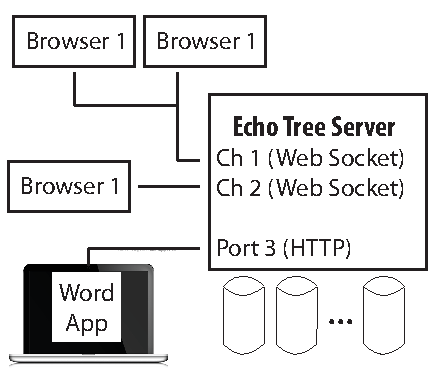
\includegraphics[width=0.5\columnwidth]{Figs/echoTreeArch.pdf}
   \caption{EchoTree architecture. Channels are implemented as
     WebSocket ports. Browsers tune in to different EchoTree channels.}
   \label{fig:arch}
\end{figure}
Central, or distributed EchoTree servers each manage some number of
distinct EchoTree channels. All facilities described above operate on
one channel. That is all shared EchoTree views are refreshed on that
channel, and requests for re-rooting occur on that channel. The server
computes trees, given a root word. Once computed, the new tree is
pushed to all subscribers.

Multiple, unrelated EchoTree sequences may be served by a single
server, using different ports. In Figure~\ref{fig:arch} Browser three
is separated from Browsers one and two, which share mutual EchoTree
transmissions.

Browsers communicate with EchoTree servers via WebSocket connections,
which are bi-directional. This bidirectionality enables the re-rooting
requests from browsers back to the server.

Figure~\ref{fig:arch} also shows an HTTP port family. These ports are
used to push new root words to the echo server from sources other than
browsers. Non-standard, desktop based text input applications for
disabled typists do not feature Web socket capabilities. The ports can
be used instead via standard socket operations. The server listening
on those ports interacts with the applications (or bridges to the
applications) via the same protocol as the browsers use over Web
sockets.  

Like new trees created in response to re-rooting requests from
browsers, the trees created in response to applications' requests
trigger the multicast of a new EchoTree to all browsers on the
respective channel. This method allows typists to focus on operating
in their usual environment, not being forced to interact with a
browser's {\em New Word} entry to push new root words.

At its bottom, Figure~\ref{fig:arch} shows a series of databases with
word follower frequencies that are the basis for the generation of the
trees. The resources in these databases consist of {\em ngrams} with
associated occurrence probabilities. That is, each database holds one
or more lists of entries consisting of a probability $p$, and two or
more words, $w_0$, $w_1$, $w_2\cdots$

For example, one snippet of such a list might look like this:

\begin{verbatim}
     1.294000e-05,circumstances,like
     1.294000e-05,He,just
     1.050000e-04,while,I
     1.294000e-05,caused,when
     1.294000e-05,not,He
\end{verbatim}

The probability informs the EchoTree construction how likely it is
that the sequence $w_1$, $w_2\cdots$ follows $w_0$. The probabilities
originate from any text collection. But as we will show, the
collections, and the choice of ngram arity have important impacts on
the generated trees. The EchoTree of Figure~\ref{fig:todayTree}, for
example, is based on bigrams from the Enron email collection
~\cite{enron}.

Given a new root word, the EchoTree constructor queries one of the
underlying databases for the top five list entries whose $w_0$ is the
root word. The choice of which list is consulted is determined by the
channel through which the re-root request was delivered, that is on
the originating subscription.

Each probability/ngram list is constructed once from one textual
source, using the Good-Turing
procedure~\cite{Gale95good-turingsmoothing}. This treatment smoothes the
otherwise spikey ngram distribution, and sets aside some probability
mass for ngrams not encountered in the underlying collection.

Cornerstones of EchoTree's system level design are the choices of
underlying data sources. But other system level desicions impact the
user experience as well. While we address the data source decision in
this paper, the following section points to some of these additional
considerations.

\section{Design Considerations}

We now illustrate how the language model that generates EchoTrees
plays into the user experience. As one more example for the details
that must be considered, we then look at the issue of stopword
removal, to be followed by a section on data source issues that
takes us to the associated experiment.

\subsection{Language Model}
The EchoTree word predictions are based on a model of the English
language. Working with ngrams has served us well. Both bigrams and
trigrams are common choices in Natural Language Processing. Both
options produce plausible word trees, but the display is by necessity
more cluttered when trigrams are shown. Figure~\ref{fig:biTrigrams}
shows a comparison between the two options, using the same root word,
{\em night.}
\begin{figure}
   \centering
   \includegraphics[width=\columnwidth]{Figs/biAndTrigrams.png}
   \caption{Comparing bigram and trigram tree displays.}
   \label{fig:biTrigrams}
\end{figure}
The trigram tree is more expressive than the bigram tree, but it is
visually denser. To a disabled typist, finding a word in the trigram
display with the intention of then transfering it to the sentence box
is more time consuming than scanning the bigram version. Depending on
the length of the sought word, the distraction time away from the
onscreen keyboard may outweigh the savings in typing.

The distraction time not only comprises the time it takes to visually
scan the tree, and to move the cursor to a found word via, for
example, a head tracker. But the onscreen keyboard must then be
re-acquired for further typing. 

Word length, which determines how profitable a cursor excursion to an
EchoTree might be, in turn is related to another design choice, the
retention or elimination of stop words.

\subsection{Stopwords}

When designing information retrieval facilities, certain very
frequently occurring words are often disregarded in user queries, and
in underlying index structures. These {\em stopwords} include words
like `the', `that', and `a'. Is stopword elimination appropriate for
our purpose of collaborative conversation? We experimented with both
options, and included examples for both in the
figures. Figure~\ref{fig:echoTree} was created while retaining
stopwords, while Figure~\ref{fig:todayTree} was constructed with
stopwords removed.

Clearly, stopword removal tends to display more interesting
words. However, the more complete sentence structure borne from
stopword retention makes it easier for conversation partners to call
out the next word choice, thus saving the disabled typist time, albeit
often for short words. Note that this time saving is enjoyed in full,
because the typist's attention can continue to dwell on the onscreen
keyboard. Short of a formal study, we have anecdotal evidence from
Henry, who prefers to lay down all words, not leaving out stopwords in
spite of the increased communication expense. A final decision on the
stopword question awaits a study.

\subsection{Data Source}

As described, the probability of any word following another is derived
from word occurrence statistics in an underlying data source. Which
source to use? Intuitively, we might suspect that using a person's own
written materials for the ngram statistics will be particularly
effective in predicting that person's writing.

Three problems arise from this approach. For one, a disabled person's
email messages, for example, will tend to be concise. This brevity in
turn limits the amount of material over which ngrams can be computed.

A second problem with using personal writing, like email, is that
obtaining the email collection is more difficult now that the material
is stored on company servers, than when email was on everyone's
personal disk. Not many email users would know how to download their
entire email history from their email provider's server. In any event,
such a startup effort is unfortunate for any computer application.

Finally, a third drawback of using personal writings is that EchoTrees
can be quite revealing. The frequency with which a particular word
follows another in one's entire personal corpus should not necessarily
be open to public view.

At the other extreme, we can use a broad source, like Google's
terabyte ngram collection \cite{google1T}. Its coverage across
millions of Web pages is more or less topic neutral, and thereby maybe
universally applicable. Between these extremes lies the option of
utilizing multiple ngram sets, each from one topic specific collection
of Web pages. When requesting re-rooting, users would choose a
configuration that is appropriately close to their topic of
conversation. Maybe the topic specificity would be beneficial.

Or, one might argue that neither email, nor Web content, nor ngrams
from scanned books \cite{anc} are optimal for a conversational
context. What if our word choices in conversations is very different
from those of our Web pages or email messages?

We conducted an experiment that examined the EchoTree performance of
three datasources, each tested under both bigram and trigram design
variants.

\section{Langage Model Evaluation}

The EchoTree system utilizes an ngram-based model trained on a corpus of sentences. In this section, we evaluate the performance of models built under several conditions. Specifically, we test the performance of bigram vs. trigram trees trained on one of three reference corpora (one of which was drawn from a corpus of Henry's writing), giving a total of six experimental conditions. 

We evaluate performance using two dependent measures relevant to the target task -- prediction reliability and saved typing time -- detailed in the following subsection. Despite the smaller size of the personal corpus, we hypothesized that the presence of a consistent author would lead to better performance for models trained on these data.

\subsection{Data Sources}
{\em Web}: 10M web pages retrieved from the {\em Recreation} section of the Open Directory Project (ODP)~\cite{dmoz}, a collaboratively-curated web directory. We eliminated all pages linked directly from the ODP site, retaining pages one-level deep in the Recreation target sites. HTML and JavaScript was removed from the pages and the text was tokenized using the Stanford NLP Tokenizer~\cite{tokenizer}, producing 5,055,284 bigrams and 28,423,891 trigrams after setting aside 10\% as a test set.

{\em Fisher}: 11,000 transcripts of ten-minute telephone conversations~\cite{fisher1,fisher2}. Each conversation centers around one topic, which was assigned to the paid participants in the conversation dyad. Metadata was removed and the text was tokenized, producing 149,789 bigrams and 93,534 trigrams after setting aside 10\% to test.

{\em Personal}: 1,167 sentences (96.5 MB) extracted from a blog maintained by our collaborator, Henry, captured on May 10, 2013~\cite{henryBlog}. This corpus produced 12,222 bigrams and 16,567 trigrams after setting aside 5\% to test.

\subsection{Performance Metrics}

The first performance component we computed for each experimental
condition is the {\em reliability} with which EchoTrees predict
follow-on words for each successive word in test sentences. The test
sentences for each condition were taken from collection set-asides of
the condition's data source. No ngrams were collected from those
set-asides. 

In measuring the reliability of an experimental condition, our
automated evaluation pulled one word $w$ after another from each
testing sentence $S$, and constructed an EchoTree with $w$ as its
root. If $w$'s follower appeared in the tree at the tree's first
level, the sentence was assigned one point. If the follower appeared
at the second tree level, one half point was awarded to the
sentence. The reliability measure for $S$ was computed as the sum of
awarded points, normalized to the length of the sentence. The data
source's single reliability performance measure is the average of the
individual sentence performances. More formally:

\begin{algorithmic}
  \FORALL{sentence $S$ in test sentences}
     \FORALL{word $w_i$ in $S$}
        \STATE tree = computeEchoTree($w_i$);
        \IF{$w_{i+1}$ in first level of tree}
            \STATE $score_s += 1$;
        \ELSIF{$w_{i+1}$ in second level of tree}
            \STATE $score_s += 0.5$;
        \ENDIF
     \ENDFOR
     \STATE normalize $score$ by length($S$);
  \ENDFOR
  \STATE $reliability = \sum_s score_s / numSentences$;
\end{algorithmic}            

The second performance measure estimates the {\em savings} in
typing. This measure is the percentage of characters that would not
need to be typed in a real life situation, because the respective
words were available in EchoTrees. We counted spaces between words in
the grand sum of letters to be typed. We also counted the click needed to
cause words in the EchoTree to replicate down into the sentence box as
a cost equivalent to typing one character. We did not consider the
time required for acquiring a word in the tree, and then re-acquiring
the onscreen keyboard.

\subsection{Procedure}
The six experimental conditions arise from the combination of three corpus conditions (Web, Fisher, and Personal) and two ngram conditions (bigram and trigram). 60 sentences were randomly selected from the set-aside test set and tokenized to generate bigrams. 

Using the procedure described in the Performance Metrics section, word trees were computed repeatedly for each word in the test sentence and then scored. This procedure produced a {\em csv} file with one line for each sentence, recording the two performance scores: typing savings (expressed as a percentage) and reliability in predicting subsequent words.

\section{Results}
We used a one-way ANOVA to evaluate the differences among mean typing savings (first dependent variable) and among mean prediction reliabilities (second dependent variable) for the six experimental conditions. Although Levene’s test found variances among the six groups to be different, we nevertheless opted for an ANOVA because our sample sizes were all equal (60 sentences).

We found a highly significant effect of the data source on savings in typing, $F(5,354)=16.0$, $p<.001$. These results are shown in Figure 6. The effect of data source on prediction reliability was also highly significant, $F(5,354)=25.4$,
$p<.001$. These results are shown in Figure 7. Tukey HSD post-hoc tests revealed a number of significant between-group differences; these are shown in Tables 1 and 2.

% Temporarily make math mode smaller for the material in the following
% tables:
\begingroup
\everymath{\scriptstyle}
\tiny

\begin{table*}
    \centering
    \begin{tabular}{|r|c|c|c|c|c|c|}
    \hline
    ~ & $Personal_{bi}$ & $Personal_{tri}$ & $Speech_{bi}$ & $Speech_{tri}$ & $Web_{bi}$ & $Web_{tri}$ \\
    ~ & $M=14.0$ & $M=12.1$ & $M=6.6$  & $M=10.1$ & $M=4.0$  & $M=11.3$ \\ 
    ~ & $SD=9.8$ & $SD=8.4$ & $SD=7.5$ & $SD=8.0$ & $SD=3.5$ & $SD=5.3$ \\ \hline
    $Personal_{bi};M=14.0,SD=9.8$  & ~                                            & ~                                             & $p<.001$                                  & $p<.045$                                    & $p<.001$                               & ~                                        \\ \hline
    $Personal_{tri};M=12.1,SD=8.4$ & ~                                            & ~                                             & $p<.05$                                   & ~                                           & $p<.001$                               & ~                                        \\ \hline
    $Speech_{bi};M=6.6,SD=7.5$     & $p<.001$                                     & $p<.05$                                       & ~                                         & ~                                           & ~                                      & $p<.05$                                  \\ \hline
    $Speech_{tri};M=10.1,SD=8.0$   & $p<.05$                                      & ~                                             & ~                                         & ~                                           & $p<.001$                               & ~                                        \\ \hline
    $Web_{bi};M=4.0,SD=3.5$        & $p<.001$                                     & $p<.001$                                      & ~                                         & $p<.001$                                    & ~                                      & $p<.001$                                 \\ \hline
    $Web_{tri};M=11.3,SD=5.3$      & ~                                            & ~                                             & $p<.05$                                   & ~                                           & $p<.001$                               & ~                                        \\ \hline
    \end{tabular}
    \caption {Post-hoc test results for savings in typing.}
    \label{tab:savings}
\end{table*}

\begin{table*}
    \centering
    \begin{tabular}{|r|c|c|c|c|c|c|}
    \hline
    ~ & $Personal_{bi}$ & $Personal_{tri}$ & $Speech_{bi}$ & $Speech_{tri}$ & $Web_{bi}$ & $Web_{tri}$ \\
    ~ & $M=.237$ & $M=.190$ & $M=.085$ & $M=.010$ & $M=.053$ & $M=.172$ \\
    ~ & $SD=.145$ & $SD=.119$ & $SD=.143$ & $SD=.091$ & $SD=.052$ & $SD=.082$ \\ \hline
    personal bi $M=.237,SD=.145$  & ~           & ~            & $p<.001$  & $p<.001$   & $p<.001$ & $p<.05$  \\ \hline
    personal tri $M=.190,SD=.119$ & ~           & ~            & $p<.001$  & $p<.001$   & $p<.001$ & ~        \\ \hline
    speech bi $M=.085,SD=.143$    & $p<.001$    & $p<.001$     & ~         & ~          & ~        & $p<.001$ \\ \hline
    speech tri $M=.010,SD=.091$   & $p<.001$    & $p<.001$     & ~         & ~          & ~        & $p<.05$  \\ \hline
    web bi $M=.053,SD=.052$       & $p<.001$    & $p<.001$     & ~         & ~          & ~        & $p<.001$ \\ \hline
    web tri $M=.172,SD=.082$       & $p<.05$     & ~            & $p<.001$  & $p<.05$    & $p<.001$ & ~        \\ \hline
    \end{tabular}
    \caption {Post-hoc test results for prediction reliability.}
    \label{tab:reliability}
\end{table*}

\endgroup

\begin{figure}
   \centering
   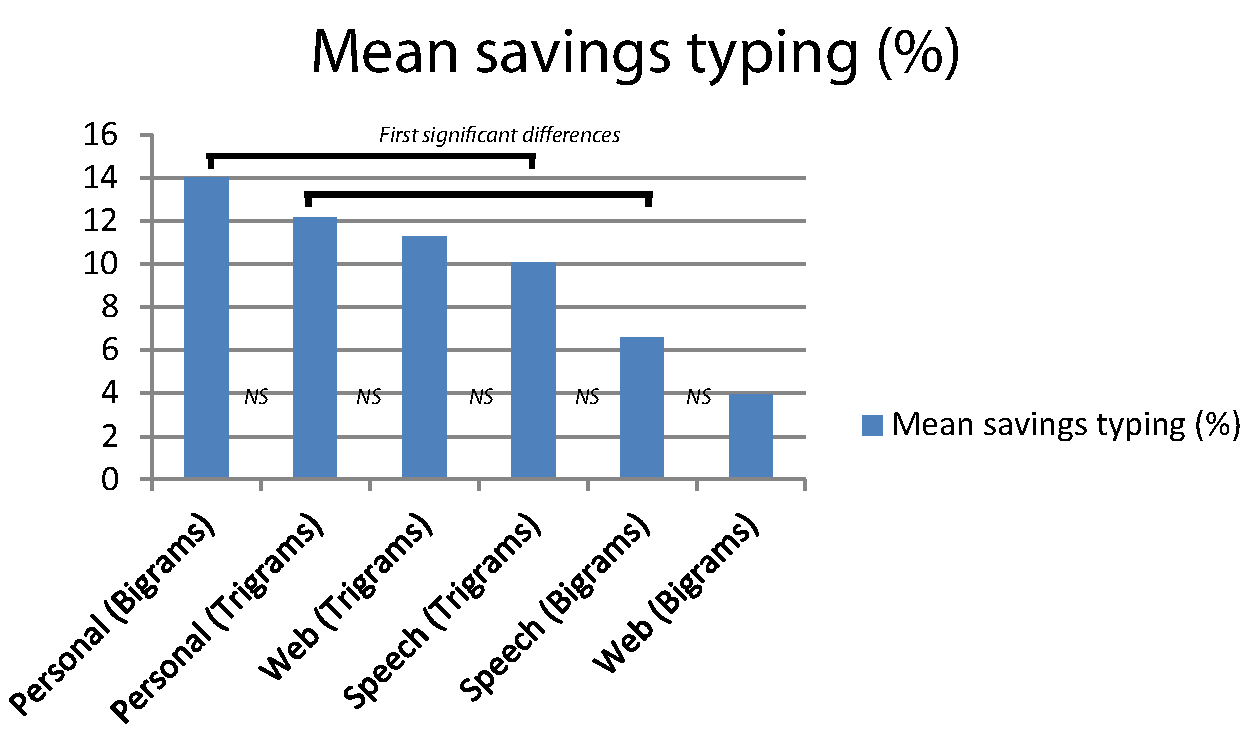
\includegraphics[width=\columnwidth]{Figs/typingSavingsChart.pdf}
   \caption{Mean savings in typing. No neighboring differences are
     significant ({\em ns})}
   \label{fig:savings}
\end{figure}

\begin{figure}
   \centering
   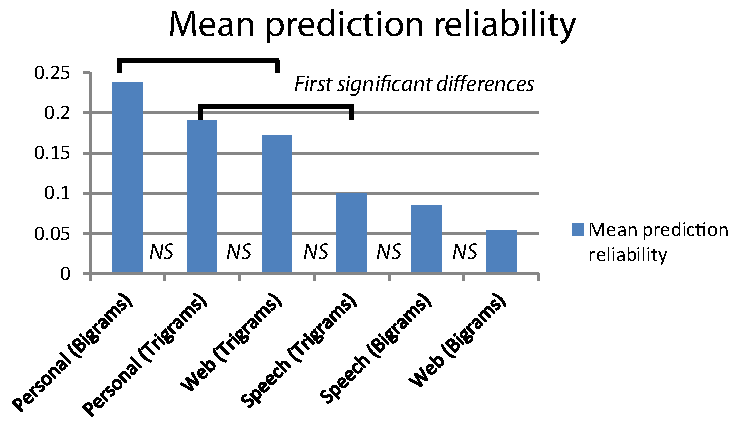
\includegraphics[width=\columnwidth]{Figs/meanPrediction.pdf}
   \caption{Mean prediction reliability. No neighboring differences are
     significant ({\em ns})}
   \label{fig:reliability}
\end{figure}

As evaluated by both performance metrics, ngrams drawn from the personal corpus performed best. However, as shown in Figure 6, most of the differences between models were not significant; $Personal_{bi}$ significantly outperformed $Speech_{tri}$, $Speech_{bi}$, and $Web_{bi}$, while $Personal_{tri}$ only outperformed $Speech_{bi}$ and $Web_{bi}$. Generally, the results show that bigrams may not be the best option, unless there is a personal reference corpus on which to train. For trigrams, results were similar for $Web_{tri}$ and $Personal_{tri}$, arguing for the use of trigrams in the case that a personal reference corpus is not available.

We were surprised by the relative strength of $Web_{tri}$. (Note that
the difference between $Web_{tri}$ and $Web_{bi}$ is significant.). We
did not expect the Web Recreation crawl to do well for either variant,
because the raw results from a crawl are very `messy.' Even after HTML
tag removal, a large amount of formatting, and styling information is
left over. Numerous menu headings, and boilerplate materials are
present as well. We made no effort to clean the corpus beyond HTML tag
removal.

Just to ensure that the random draw of $Web_{tri}$ test sentences did
not produce an unusual outcome, we repeated $Web_{tri}$ with a
different set of random 60 sentences from the respective
set-aside. The result was comparable to Figure~\ref{fig:savings}.

The prediction reliability (Figure~\ref{fig:reliability}) shows that
the order of the six conditions by decreasing performance is as per the
savings measure. A fundamental difference between the two measures,
however, is that reliability does not depend on individual word
lengths. 

The best performer in reliability was $Personal_{bi}$ with just under
.25 on the scale from 0 to 1. Again, for bigram trees no choice is
better than $Personal_{bi}$. The next bigram choice is $Speech_{bi}$,
which is a significantly worse performer for prediction. For trigrams,
however, the equivalent choice of $Web_{tri}$ is available.

In summary, the optimal choice for ngram data source is always the
personal collection. This result holds for both bigram and trigram
trees. 

For bigrams, the next best choice is to use the Fisher
conversation transcripts, albeit at large cost in typing savings and
prediction reliability.

If trigrams are acceptable to end users, then the recreation Web crawl
is an acceptable choice for both savings and reliability.

\section{Discussion}

Our experiments with various data sources find that a bigram model based on the user's own communication data performs best with respect to prediction reliability and overall typing saved. In the absence of such a personal corpus, we have found that a trigram model trained on a web corpus of recreation pages performs reasonably well. Starting with such a web corpus and capturing communication through continued use of the system may serve as a valauble bootstrapping method for developing a personal corpus.

Our findings suggest possible design choices for improving our language model. We first note the high performance of the $Web_{tri}$ corpus, biased towards a single topic, compared to the Fisher corpus, which ranges over many topics. Allowing the typist to choose from several topic-specific corpora based on conversation topic could lead to performance gains. For this reason, the EchoTree architecture (Figure~\ref{fig:arch}) anticipates multiple ngram sources that can be switched dynamically. EchoTree could also be improved by techniques draw from the domain of natural language processing. Word stemming, for instance, would likely lead to improvements in prediction reliability, as well as identification of syntactic structures. Adding a learning component, such that ngram weights are adjusted for each user over time, could provide long-term gains, as well.

Clearly, end-user experiments are required as well to resolve at least two questions. First, are bigram or trigram trees the preferred visual representation for supporting conversations with the impaired typist? Improving comprehensibility on the conversation partner’s end will surely improve the quality of predictions and generation of rapport. Second, do conversation partners generate correct guesses that capture the typist’s intention but which differ from the literal suggestions given by EchoTree? If such associative guesses do occur, then the overall system -- machine plus human(s) -- could exceed the performance measures seen in our experiment.

\section{Related Work}

Though our work was motivated by a desire to improve Henry's ability to converse, he is not alone in his needs as an individual with impaired speech. In the United States alone, roughly 2.8M people (1.2\%) reported difficulty with speech in 2010, of which 523,000 (0.2%) reported severe difficulties. EchoTree falls into a long line of research in the area of {\em Augmented and Alternative Communication} (AAC) focused on adapting developments in communication technologies to improve the rate, fluidity, and efficacy of communication for users with physical or speech impairments~\cite{vanderheiden2002}.

Advances in language modeling and prediction have been fruitful for
AAC researchers; anticipating imminent letters, words, or even
sentences can vastly reduce text input demands of impaired
users. Systems such as Humsher~\cite{Polacek2011}, for example, have
adapted letter-based text-entry systems developed for able-bodied
users to significantly accelerate text entry for severely
motor-impaired users. 

Past research on n-gram prediction-based AAC systems has shown that the additional cognitive overhead imposed by having to monitor predictions can actually outweigh the typing savings, leading to slower communication overall~\cite{venkatagiri1993, koester1994}. In a study aimed at addressing this issue, Trnka et al. stress the importance of the quality of the predictive model in overcoming this tradeoff~\cite{Trnka2009}. For this reason, we focus our evaluation in this paper on optimizing aspects related to the language model, before conducting the user evalautions planned for future work.

EchoTree builds not only on prior research in n-gram word prediction,
but also on prior work in technology-assisted co-construction of
sentences. Prior efforts have shown how involving an able-bodied
communication partner in the conversation loop to make guesses about
the intended messages can complement the benefits offered by ngram
language models~\cite{Roark2011}. 

Similarly, the visual design of EchoTree adapts the interactive
"keyword-in-context" visualization technique embodied in the Word
tree~\cite{Wattenberg2008} from its original purpose of retrospective
corpus studies to the new problem of collaborative text
generation. The use of visual metaphors, direct interaction, and
output-as-input techniques allow for tight coupling between
conversation participants and the information
display~\cite{Ahlberg1994}. EchoTree's sentence box and confirmation
loop further afford the process of grounding, enabling tighter
coupling between the conversation partners themselves as they
negotiate the evolving sentence together.~\cite{clark1991}.

% Without the following linebreak encouragement,
% we get 'Conclusion' on one page, and the body
% of the section on the next:
\section{Conclusion}
In this paper, we introduced EchoTrees, a language modeling and visualization approach designed to engage conversation partners and faciltiate the speed and quality of communication for motion and speech-impaired users. As the impaired user types words, the past sentence context is displayed along with a WordTree visualizing likely possible future words. Our implementation of this approach as a browser-based application allows co-located or remote participants to view and select possible upcoming words, thus saving the typist time and effort. We discussed the design considerations and implementation details of our system, as well as the results of empirical evaluation of various data sources aimed at identifying the best means for constructing language models in this interactive conversation scenario.

The problem of social isolation for communication-impaired individuals is clearly difficult to solve in the general case. However, through the design of EchoTree, we demonstrate that specialized computer-supported collaborative solutions can ameliorate some of the problems associated with this isolation. Computers are patient where conversation partners are not. By connecting the individual, the computer, and the conversation partners in an interactive loop, EchoTree can facilitate a more efficient, more enjoyable, and less isolating experience for users such as Henry.

%**********************
%   - user studies for guessing
%   - broadcast each letter as Henry types
%   - hybrid data sources: general with personal information injected
%   - get reliability higher

%% \section{Acknowledgments}
%% Thank you to Henry (anonymized for submission) for patient testing,
%% and encouragment of crazy ideas. And: we are grateful to (anonymous)
%% for his JavaScript prowess, and willingness to apply it.
%-------------------


% Balancing columns in a ref list is a bit of a pain because you
% either use a hack like flushend or balance, or manually insert
% a column break.  http://www.tex.ac.uk/cgi-bin/texfaq2html?label=balance
% multicols doesn't work because we're already in two-column mode,
% and flushend isn't awesome, so I choose balance.  See this
% for more info: http://cs.brown.edu/system/software/latex/doc/balance.pdf
%
% Note that in a perfect world balance wants to be in the first
% column of the last page.
%
% If balance doesn't work for you, you can remove that and
% hard-code a column break into the bbl file right before you
% submit:
%
% http://stackoverflow.com/questions/2149854/how-to-manually-equalize-columns-
% in-an-ieee-paper-if-using-bibtex
%
% Or, just remove \balance and give up on balancing the last page.
%
\balance

% If you want to use smaller typesetting for the reference list,
% uncomment the following line:
% \small
\bibliographystyle{acm-sigchi}
\scriptsize{\bibliography{echoTree}}
\end{document}
